%-----------------------------------------------------------------------------------------------------------------------------------------------%
%	The MIT License (MIT)
%
%	Copyright (c) 2019 Jan Küster
%
%	Permission is hereby granted, free of charge, to any person obtaining a copy
%	of this software and associated documentation files (the "Software"), to deal
%	in the Software without restriction, including without limitation the rights
%	to use, copy, modify, merge, publish, distribute, sublicense, and/or sell
%	copies of the Software, and to permit persons to whom the Software is
%	furnished to do so, subject to the following conditions:
%	
%	THE SOFTWARE IS PROVIDED "AS IS", WITHOUT WARRANTY OF ANY KIND, EXPRESS OR
%	IMPLIED, INCLUDING BUT NOT LIMITED TO THE WARRANTIES OF MERCHANTABILITY,
%	FITNESS FOR A PARTICULAR PURPOSE AND NONINFRINGEMENT. IN NO EVENT SHALL THE
%	AUTHORS OR COPYRIGHT HOLDERS BE LIABLE FOR ANY CLAIM, DAMAGES OR OTHER
%	LIABILITY, WHETHER IN AN ACTION OF CONTRACT, TORT OR OTHERWISE, ARISING FROM,
%	OUT OF OR IN CONNECTION WITH THE SOFTWARE OR THE USE OR OTHER DEALINGS IN
%	THE SOFTWARE.
%	
%
%-----------------------------------------------------------------------------------------------------------------------------------------------%


%============================================================================%
%
%	DOCUMENT DEFINITION
%
%============================================================================%

%we use article class because we want to fully customize the page and don't use a cv template
\documentclass[10pt,A4]{article}	


%----------------------------------------------------------------------------------------
%	ENCODING
%----------------------------------------------------------------------------------------

% we use utf8 since we want to build from any machine
\usepackage[utf8]{inputenc}		

%----------------------------------------------------------------------------------------
%	LOGIC
%----------------------------------------------------------------------------------------

% provides \isempty test
\usepackage{xstring, xifthen}

%----------------------------------------------------------------------------------------
%	FONT BASICS
%----------------------------------------------------------------------------------------

% some tex-live fonts - choose your own

%\usepackage[defaultsans]{droidsans}
%\usepackage[default]{comfortaa}
%\usepackage{cmbright}
\usepackage[default]{raleway}
%\usepackage{fetamont}
%\usepackage[default]{gillius}
%\usepackage[light,math]{iwona}
%\usepackage[thin]{roboto} 

% set font default
\renewcommand*\familydefault{\sfdefault} 	
\usepackage[T1]{fontenc}

% more font size definitions
\usepackage{moresize}

%----------------------------------------------------------------------------------------
%	FONT AWESOME ICONS
%---------------------------------------------------------------------------------------- 

% include the fontawesome icon set
\usepackage{fontawesome}

% use to vertically center content
% credits to: http://tex.stackexchange.com/questions/7219/how-to-vertically-center-two-images-next-to-each-other
\newcommand{\vcenteredinclude}[1]{\begingroup
\setbox0=\hbox{\includegraphics{#1}}%
\parbox{\wd0}{\box0}\endgroup}

% use to vertically center content
% credits to: http://tex.stackexchange.com/questions/7219/how-to-vertically-center-two-images-next-to-each-other
\newcommand*{\vcenteredhbox}[1]{\begingroup
\setbox0=\hbox{#1}\parbox{\wd0}{\box0}\endgroup}

% icon shortcut
\newcommand{\icon}[3] { 							
	\makebox(#2, #2){\textcolor{maincol}{\csname fa#1\endcsname}}
}	

% icon with text shortcut
\newcommand{\icontext}[4]{ 						
	\vcenteredhbox{\icon{#1}{#2}{#3}}  \hspace{2pt}  \parbox{0.9\mpwidth}{\textcolor{#4}{#3}}
}

% icon with website url
\newcommand{\iconhref}[5]{ 						
    \vcenteredhbox{\icon{#1}{#2}{#5}}  \hspace{2pt} \href{#4}{\textcolor{#5}{#3}}
}

% icon with email link
\newcommand{\iconemail}[5]{ 						
    \vcenteredhbox{\icon{#1}{#2}{#5}}  \hspace{2pt} \href{mailto:#4}{\textcolor{#5}{#3}}
}

%----------------------------------------------------------------------------------------
%	PAGE LAYOUT  DEFINITIONS
%----------------------------------------------------------------------------------------

% page outer frames (debug-only)
% \usepackage{showframe}		

% we use paracol to display breakable two columns
\usepackage{paracol}

% define page styles using geometry
\usepackage[a4paper]{geometry}

% remove all possible margins
\geometry{top=1cm, bottom=1cm, left=1cm, right=1cm}

\usepackage{fancyhdr}
\pagestyle{empty}

% space between header and content
% \setlength{\headheight}{0pt}

% indentation is zero
\setlength{\parindent}{0mm}

%----------------------------------------------------------------------------------------
%	TABLE /ARRAY DEFINITIONS
%---------------------------------------------------------------------------------------- 

% extended aligning of tabular cells
\usepackage{array}

% custom column right-align with fixed width
% use like p{size} but via x{size}
\newcolumntype{x}[1]{%
>{\raggedleft\hspace{0pt}}p{#1}}%


%----------------------------------------------------------------------------------------
%	GRAPHICS DEFINITIONS
%---------------------------------------------------------------------------------------- 

%for header image
\usepackage{graphicx}

% use this for floating figures
% \usepackage{wrapfig}
% \usepackage{float}
% \floatstyle{boxed} 
% \restylefloat{figure}

%for drawing graphics		
\usepackage{tikz}				
\usetikzlibrary{shapes, backgrounds,mindmap, trees}

%----------------------------------------------------------------------------------------
%	Color DEFINITIONS
%---------------------------------------------------------------------------------------- 
\usepackage{transparent}
\usepackage{color}

% primary color
\definecolor{maincol}{RGB}{ 45, 50, 90 }

% accent color, secondary
% \definecolor{accentcol}{RGB}{ 250, 150, 10 }

% dark color
\definecolor{darkcol}{RGB}{ 70, 70, 70 }

% light color
\definecolor{lightcol}{RGB}{245,245,245}


% Package for links, must be the last package used
\usepackage[hidelinks]{hyperref}

% returns minipage width minus two times \fboxsep
% to keep padding included in width calculations
% can also be used for other boxes / environments
\newcommand{\mpwidth}{\linewidth-\fboxsep-\fboxsep}
	


%============================================================================%
%
%	CV COMMANDS
%
%============================================================================%

%----------------------------------------------------------------------------------------
%	 CV LIST
%----------------------------------------------------------------------------------------

% renders a standard latex list but abstracts away the environment definition (begin/end)
\newcommand{\cvlist}[1] {
	\begin{itemize}{#1}\end{itemize}
}

%----------------------------------------------------------------------------------------
%	 CV TEXT
%----------------------------------------------------------------------------------------

% base class to wrap any text based stuff here. Renders like a paragraph.
% Allows complex commands to be passed, too.
% param 1: *any
\newcommand{\cvtext}[1] {
	\begin{tabular*}{1\mpwidth}{p{0.98\mpwidth}}
		\parbox{1\mpwidth}{#1}
	\end{tabular*}
}

%----------------------------------------------------------------------------------------
%	CV SECTION
%----------------------------------------------------------------------------------------

% Renders a a CV section headline with a nice underline in main color.
% param 1: section title
\newcommand{\cvsection}[1] {
	\vspace{14pt}
	\cvtext{
		\textbf{\LARGE{\textcolor{darkcol}{\uppercase{#1}}}}\\[-4pt]
		\textcolor{maincol}{ \rule{0.1\textwidth}{2pt} } \\
	}
}

%----------------------------------------------------------------------------------------
%	META SKILL
%----------------------------------------------------------------------------------------

% Renders a progress-bar to indicate a certain skill in percent.
% param 1: name of the skill / tech / etc.
% param 2: level (for example in years)
% param 3: percent, values range from 0 to 1
\newcommand{\cvskill}[3] {
	\begin{tabular*}{1\mpwidth}{p{0.72\mpwidth}  r}
 		\textcolor{black}{\textbf{#1}} & \textcolor{maincol}{#2}\\
	\end{tabular*}%
	
	\hspace{4pt}
	\begin{tikzpicture}[scale=1,rounded corners=2pt,very thin]
		\fill [lightcol] (0,0) rectangle (1\mpwidth, 0.15);
		\fill [maincol] (0,0) rectangle (#3\mpwidth, 0.15);
  	\end{tikzpicture}%
}


%----------------------------------------------------------------------------------------
%	 CV EVENT
%----------------------------------------------------------------------------------------

% Renders a table and a paragraph (cvtext) wrapped in a parbox (to ensure minimum content
% is glued together when a pagebreak appears).
% Additional Information can be passed in text or list form (or other environments).
% the work you did
% param 1: time-frame i.e. Sep 14 - Jan 15 etc.
% param 2:	 event name (job position etc.)
% param 3: Customer, Employer, Industry
% param 4: Short description
% param 5: work done (optional)
% param 6: technologies include (optional)
% param 7: achievements (optional)
\newcommand{\cvevent}[7] {
	
	% we wrap this part in a parbox, so title and description are not separated on a pagebreak
	% if you need more control on page breaks, remove the parbox
	\parbox{\mpwidth}{
		\begin{tabular*}{1\mpwidth}{p{0.72\mpwidth}  r}
	 		\textcolor{black}{\textbf{#2}} & \colorbox{maincol}{\makebox[0.25\mpwidth]{\textcolor{white}{#1}}} \\
			\textcolor{maincol}{\textbf{#3}} & \\
		\end{tabular*}\\[4pt]
	
		\ifthenelse{\isempty{#4}}{}{
			\cvtext{#4}\\
		}
	}

	\ifthenelse{\isempty{#5}}{}{
		\vspace{4pt}
		{#5}
	}
	\vspace{4pt}
}

%----------------------------------------------------------------------------------------
%	 CV META EVENT
%----------------------------------------------------------------------------------------

% Renders a CV event on the sidebar
% param 1: title
% param 2: subtitle (optional)
% param 3: customer, employer, etc,. (optional)
% param 4: info text (optional)
\newcommand{\cvmetaevent}[4] {
	\textcolor{maincol} {\cvtext{\textbf{\begin{flushleft}#1\end{flushleft}}}}

	\ifthenelse{\isempty{#2}}{}{
	\textcolor{darkcol} {\cvtext{\textbf{#2}} }
	}

	\ifthenelse{\isempty{#3}}{}{
		\cvtext{{ \textcolor{darkcol} {#3} }}\\
	}

	\cvtext{#4}\\[14pt]
}

%---------------------------------------------------------------------------------------
%	QR CODE
%----------------------------------------------------------------------------------------

% Renders a qrcode image (centered, relative to the parentwidth)
% param 1: percent width, from 0 to 1
\newcommand{\cvqrcode}[1] {
	\begin{center}
		\includegraphics[width={#1}\mpwidth]{qrcode}
	\end{center}
}

%=+=+=+=+=+=+=+=+=+=+=+=+=+=+=+=+=+=+=+=+=+=+=+=+=+=+=+=+=+=+=+=+=+=+=+=+=+=+=+=+
%,,,,,,,,,,,,,,,,,,,,,,,,,,,,,,,,,,,,,,,,,,,,,,,,,,,,,,,,,,,,,,,,,,,,,,,,,,,,,,,,
                       % EDIT AFTER THIS POINT
%''''''''''''''''''''''''''''''''''''''''''''''''''''''''''''''''''''''''''''''''
%=+=+=+=+=+=+=+=+=+=+=+=+=+=+=+=+=+=+=+=+=+=+=+=+=+=+=+=+=+=+=+=+=+=+=+=+=+=+=+=+


%============================================================================%
%
%
%
%	DOCUMENT CONTENT
%
%
%
%============================================================================%
\begin{document}
\columnratio{0.31}
\setlength{\columnsep}{2.2em}
\setlength{\columnseprule}{4pt}
\colseprulecolor{lightcol}
\begin{paracol}{2}
\begin{leftcolumn}
%---------------------------------------------------------------------------------------
%	META IMAGE
%----------------------------------------------------------------------------------------
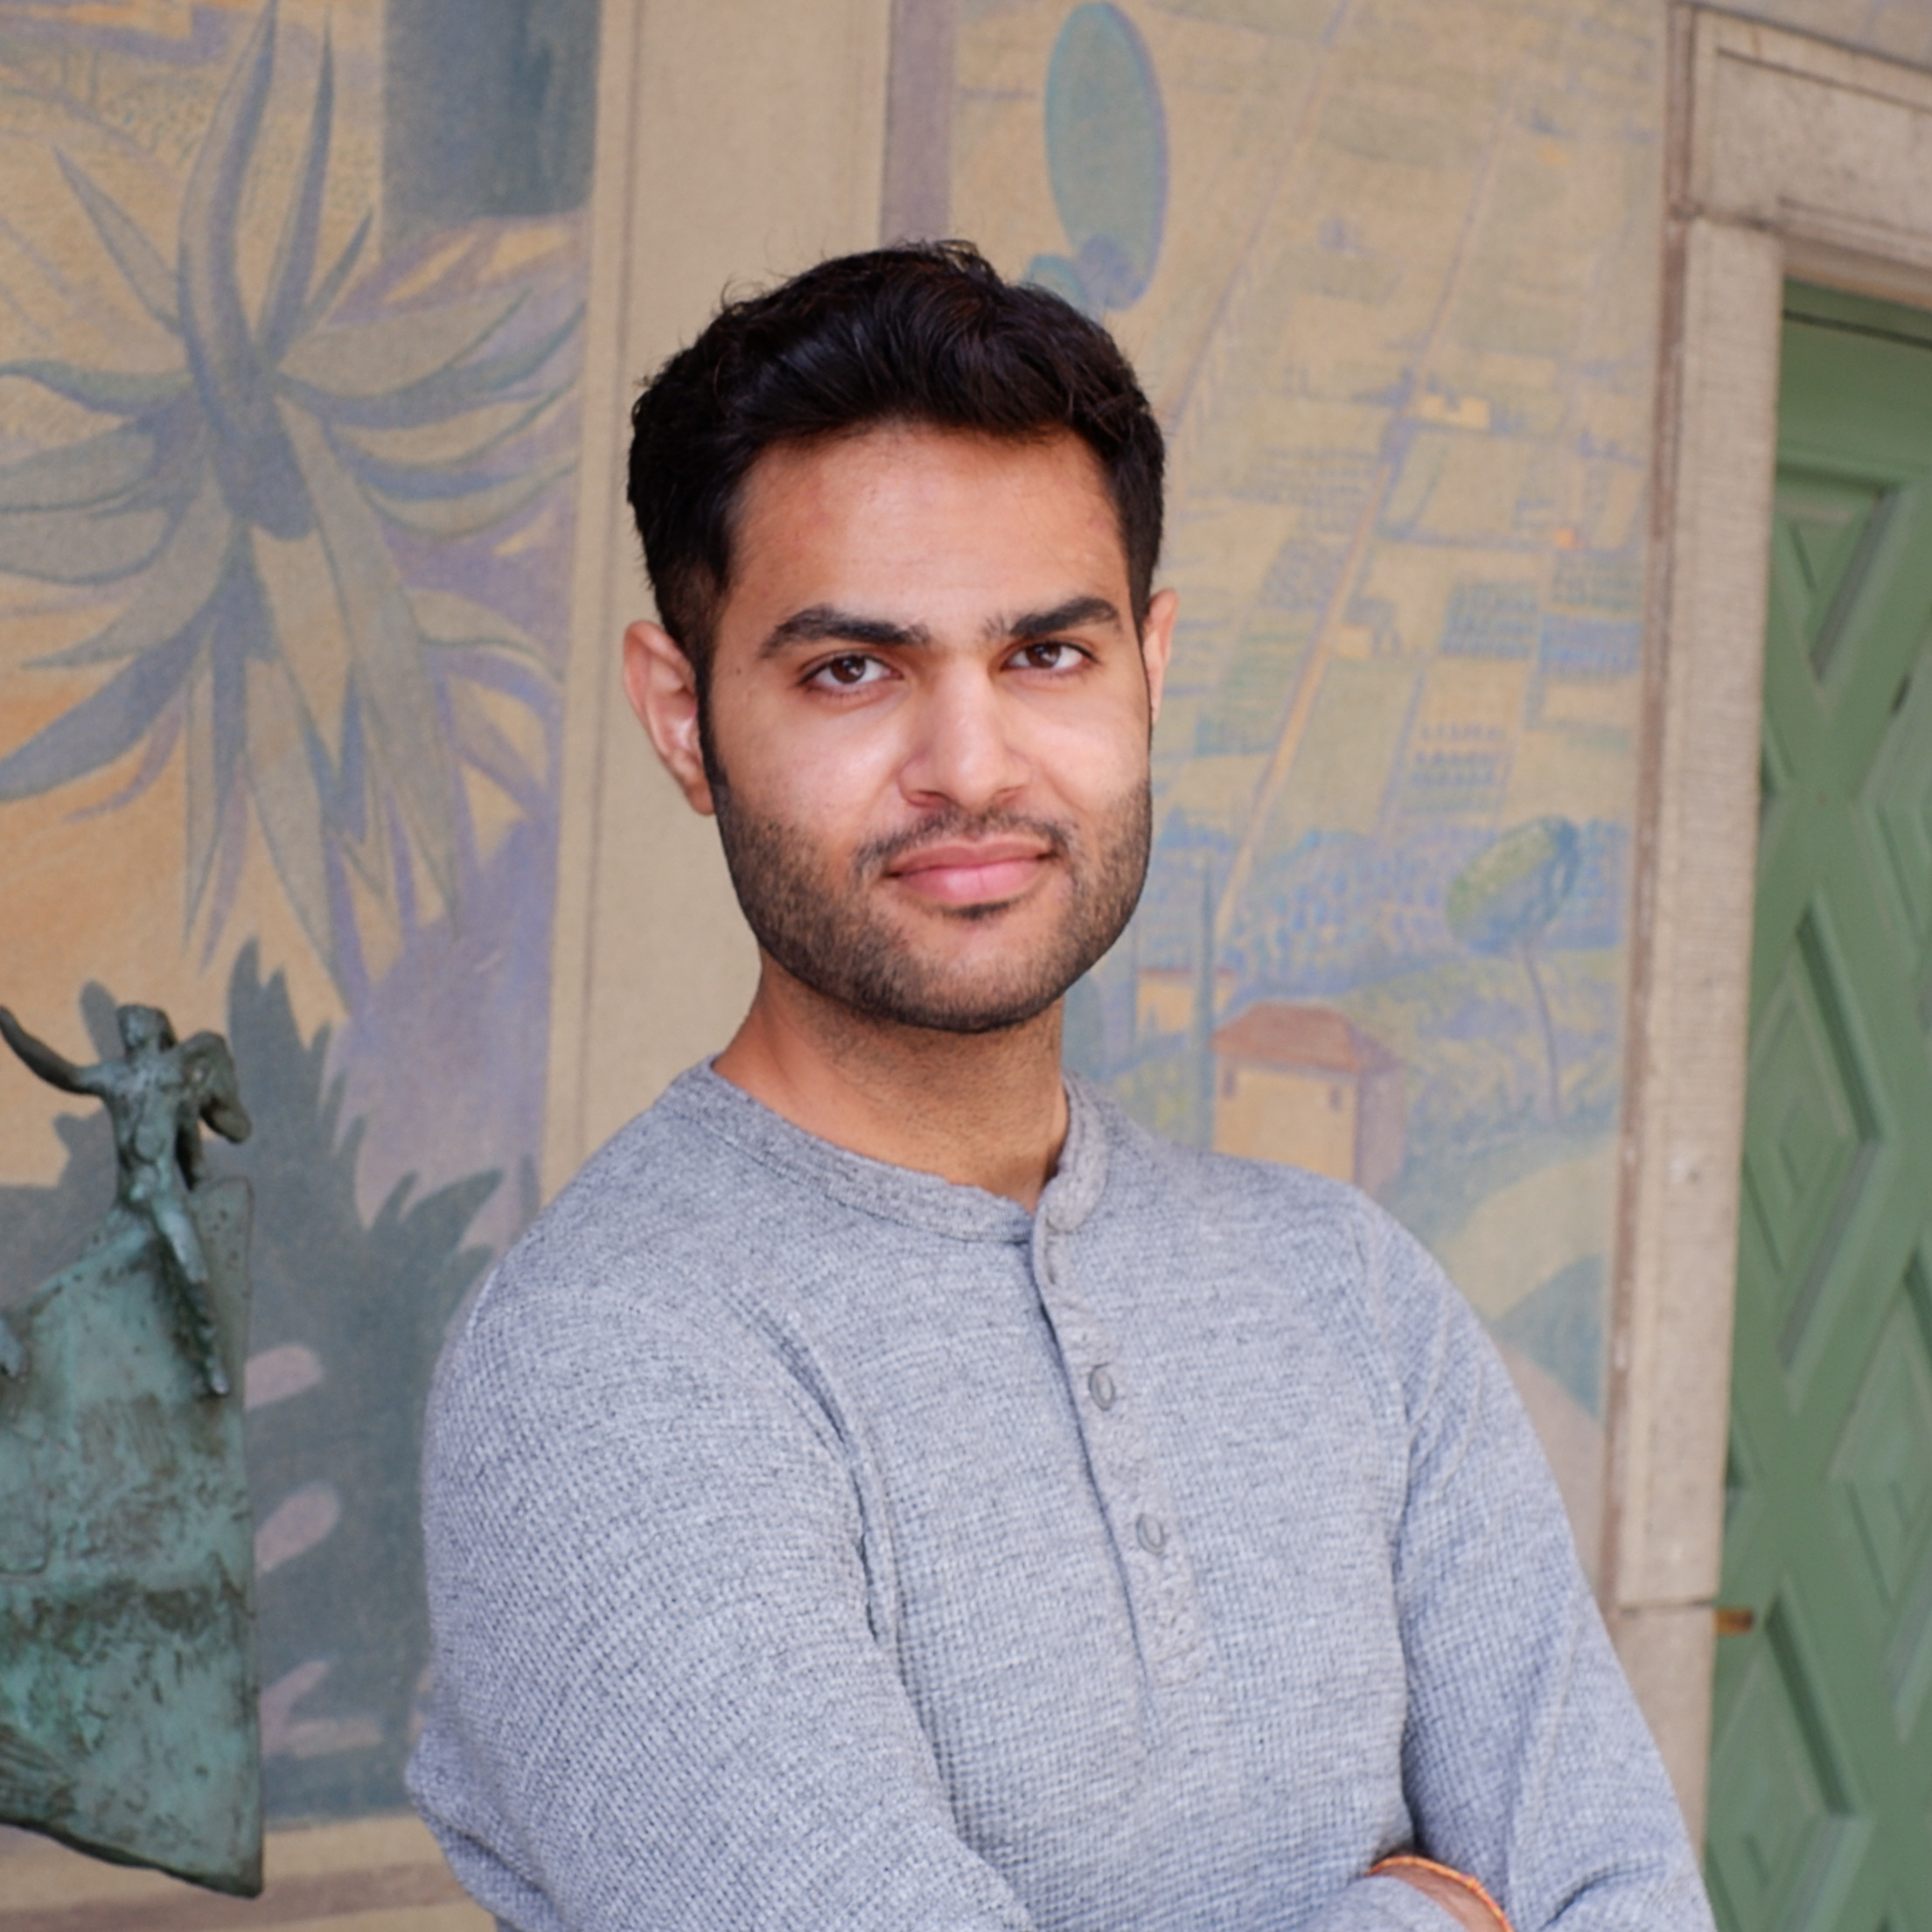
\includegraphics[width=\linewidth]{DSCF2214.JPG}	%trimming relative to image size


\vfill\null
\cvsection{CONTACT}
	
\iconemail{EnvelopeSquare}{14}{jayantyadav202@gmail.com}{jayantyadav202@gmail.com}{black}\\[6pt]
\icontext{Github}{14}{\href{https://github.com/jayant-yadav}{jayant-yadav}}{black}\\[6pt]
\icontext{Linkedin}{14}{\href{https://www.linkedin.com/in/jayant-yadav/}{jayant-yadav}}{black}\\[6pt]
\icontext{Globe}{14}{\href{https://sites.google.com/view/jayantyadav/home}{jayantyadav}}{black}\\[6pt]
\icontext{Phone}{14}{+46 764330325}{black}\\[6pt]
\icontext{Whatsapp}{14}{+91 9999157033}{black}\\[6pt]
%\faWhatsapp \hspace{2pt}{+91 9999157033}
\vfill\null
%\cvqrcode{0.7}

%---------------------------------------------------------------------------------------
%	META SKILLS
%----------------------------------------------------------------------------------------
\cvsection{SKILLS}

%\cvskill{Skill_Name} {Years of experience} {percentage of bar fill} \\[-2pt]

\cvskill{Python} {5+ yrs} {0.8} \\[-2pt]

\cvskill{C++} {3+ yrs} {0.3} \\[-2pt]

\cvskill{MySQL} {6+ yrs} {1} \\[-2pt]

\cvskill{MongoDB} {1+ yrs} {0.3} \\[-2pt]

\cvskill{Linux} {6+ yrs} {1} \\[-2pt]

\cvskill{Data Warehousing} {2+ yrs} {0.8} \\[-2pt]

\cvskill{Machine Learning} {2+ yrs} {0.7} \\[-2pt]

\cvskill{Web Development} {2+ yrs} {0.4} \\[-2pt]

\cvskill{Tableau} {2+ yrs} {1} \\[-2pt]

\cvskill{Jira/Confluence} {3+ yrs} {1} \\[-2pt]

%\vfill\null
%\cvqrcode{0.7}

%---------------------------------------------------------------------------------------
%	ACHIEVEMENTS
%----------------------------------------------------------------------------------------
\newpage
\cvsection{ACHIEVEMENTS}

\cvmetaevent
{GRE}
{318/240 (Quant- 165/170; Verbal- 153/170; AWA- 4/6)}
{}
{A standardized test that is an admissions requirement for many graduate schools in the United States and Canada and few in other countries.}

\cvmetaevent
{Spot Award}
{Deloitte India (Offices of the US)}
{}
{Special contribution accomplished over a relatively short time period and showcased technical and functional capabilities.}

\end{leftcolumn}
\begin{rightcolumn}
%---------------------------------------------------------------------------------------
%	TITLE  HEADER
%----------------------------------------------------------------------------------------
\fcolorbox{white}{darkcol}{\begin{minipage}[c][3.5cm][c]{1\mpwidth}
	\begin {center}
		\HUGE{ \textbf{ \textcolor{white}{ \uppercase{ JAYANT YADAV } } } } \\[-24pt]
		\textcolor{white}{ \rule{0.1\textwidth}{1.25pt} } \\[4pt]
		\large{ \textcolor{white} {Masters in Computer Science } }
	\end {center}
\end{minipage}} \\[14pt]
\vspace{-12pt}

%---------------------------------------------------------------------------------------
%	EDUCATION
%----------------------------------------------------------------------------------------
%\vfill\null
\cvsection{EDUCATION}

\cvevent
	{\textbf{2021 - present}}
	{Master's in Computer Science}
	{Uppsala Universitet - Uppsala (Sweden)}
	{Courses: Statistical Machine Learning, Natural Computational Methods for Machine Learning, Data Engineering, Reinforcement Learning, Data Ethics and Law and Image Analysis.}
\vfill\null

\cvevent
	{\textbf{2013 - 2017}}
	{B. Tech. - Computer Science $\&$ Engineering}
	{Jaypee Institute of Information Technology -  Noida, U.P. (India)}
	{Passed with 7.8 CGPA. Major Project Grade: A}
\vfill\null

%---------------------------------------------------------------------------------------
%	WORK EXPERIENCE
%----------------------------------------------------------------------------------------
\vfill\null
\cvsection{WORK EXPERIENCE}

\cvevent
	{\textbf{Nov 18 - Jul 21}}
	{Data Analytics Lead}
	{Dure Technologies, Thane (Maharashtra)}
	{
	\begin{itemize}
	%E-mobility project:
\item Managed a team of 5, responsible of analyzing data on 100K+ EV charging stations and 30M+ charging sessions for 90+ countries. Inferred valuable business insights by constructing ETL pipelines, Data warehouse and recommendation engine using python, MySQL, Tableau and geo-spatial open-source data.
% COVID and other public health projects:
\item Worked with ICMR and WHO to help Govt of India prepare for the National and Sub-National Covid Response by helping create predictive models around Covid Wave preparedness and capacity planning.
\item Developed multi-disease monitoring Analytical platform for TB, HIV for global, national and sub-national stakeholders using heatmaps, butterfly charts, state diagrams, decomposition trees, etc. based on the data provided by countries, open data and derived information.
	\end{itemize}
	}
	{}
\vfill\null

\cvevent
	{\textbf{Jul 17 - Oct 18}}
	{Advisory Analyst}
	{Deloitte USI, Hyderabad (Telangana)}
	{
	\begin{itemize}
	    \item Monitored Real-time threats, incidents of potential intrusions and performed triage of events through SIEM Tools namely LogRhythm, Splunk and IBM Qradar. Raised critical cases to the client within the time frame of SLA.
        \item  Worked on multiple endpoint security tools such as Carbon Black, Symantec Endpoint Protection, Proofpoint and Fidelis.
	\end{itemize}
	}
	{}
\vfill\null

\cvevent
	{\textbf{Oct 16 - May 17}}
	{Web Developer}
	{Mozilla Winter of Security, Mozilla (Remote)}
	{Worked on a web interface for Mozilla Investigator (MIG), which is primarily a command-line tool, as part of Mozilla Winter of Security 2016; integrated MIG API (built in golang) with AngularJS.}
	{}
\vfill\null


\cvevent
	{\textbf{Jun 16 - Aug 16}}
	{Web Developer}
	{VisoinITLabs, New Delhi (Delhi)}
	{
	\begin{itemize}
	    \item Full stack development of teacher's test preparation portal, to assist faculties to prepare the academy's test papers more conveniently.
        \item Suggested changes to the company's database.
	\end{itemize}
}
	{}
\vfill\null

%---------------------------------------------------------------------------------------
%	PUBLICATION
%----------------------------------------------------------------------------------------
\vspace{-0.5cm}
\vfill\null
\cvsection{PUBLICATIONS}

\cvevent
	{\textbf{IEEE}}
	{Diabetic Retinopathy Detection using feedforward Neural Network}
	{2017 Tenth International Conference on Contemporary Computing (IC3) (ISSN: 2572-6129) DOI: 10.1109/IC3.2017.8284350}
	{Status: Accepted and Published}
	{}
\vfill\null

%---------------------------------------------------------------------------------------
%	PROJECTS
%----------------------------------------------------------------------------------------
\vfill\null
\cvsection{PROJECTS}

\cvevent
	{\textbf{2022}}
	{Github Analytics using Pulsar}
	{Tool: Apache Pulsar, MongoDB, Docker, CloudInit}
	{Developed an analytic system for GitHub using Github API and streaming framework, Apache pulsar. The system was scalable, could contextualize multiple nodes to fetch data parallely and store it in MongoDB, further allowing adaptive queries to be run on the database.}
\vfill\null


\cvevent
	{\textbf{2022}}
	{Multi-genre classification of movies}
	{Tool: PyTorch, Transfer learning}
	{Performed a multi-label classification of images on movie posters. Trained a neural network based on modified DenseNet architecture and a custom CNN using PyTorch on 20 different movie genres. }
\vfill\null


\cvevent
	{\textbf{2021}}
	{Do (wo)men talk too much in films?}
	{Tool: python, scikit-learn, pandas}
	{Aimed at measuring whether the male or female lead role is predictable from the amount of dialogue the actors have, the year the film was made, how much money it made and so on. Performed EDA and  trained supervised ML models like Logistic Regression, LDA, QDA, KNN, Random forest and Gradient boosting.}
\vfill\null

%---------------------------------------------------------------------------------------
%	WORKSHOPS
%----------------------------------------------------------------------------------------
%\vfill\null
%\cvsection{WORKSHOPS \& CONFERENCES}

%\cvevent
%	{\textbf{Mon 20XX}}
%	{Name of Conference}
%	{Conducted by}
%	{}
%\vfill\null

%\cvevent
%	{\textbf{May 2019}}
%	{IEEE Internation Conference on Future of Internet of Things}
%	{IEEE \& IIT Kanpur}
%	{}
%\vfill\null

%\cvevent
%	{\textbf{Jul 2020}}
%	{Online International Workshop on Machine Learning Applications to Images, IoT and Wireless Sensor Networks}
%	{University of Essex and IIIT, Lucknow}
%	{}
%\vfill\null

%---------------------------------------------------------------------------------------
%	SKILLS
%----------------------------------------------------------------------------------------

%---------------------------------------------------------------------------------------
%	PERSONAL DETAILS
%----------------------------------------------------------------------------------------
\vfill\null
\cvsection{EXTRACURRICULAR}
\vspace{-0.3cm}
\begin{itemize}

  \item Member of Photography club at Kalmar Nation, Uppsala University. 
  \item Watches random science videos, anime, psychology and neuroscience podcasts.
  \item Vice President of Delhi Aspire, Rotaract Club RID 3012, a humanitarian service organization, part of Rotary International youth program.
  \item First and second position in two separate autonomous and manual robotics events conducted at college (2014).
  \item First position in inter-college football competition 2017 having the participation of 10+ teams.

\end{itemize}
\vfill\null


\vfill
\vfill
\vfill
\end{rightcolumn}
\end{paracol}
\end{document}

